% 原始嵌入曲线位图，原图位置上的中文标签由 TikZ 排印。
\begin{figure}[htbp]
\centering
\begin{tikzpicture}[x=0.08mm,y=-0.08mm,inner sep=0pt]
\node[anchor=north west] (ch01dfig16data) at (0,0) {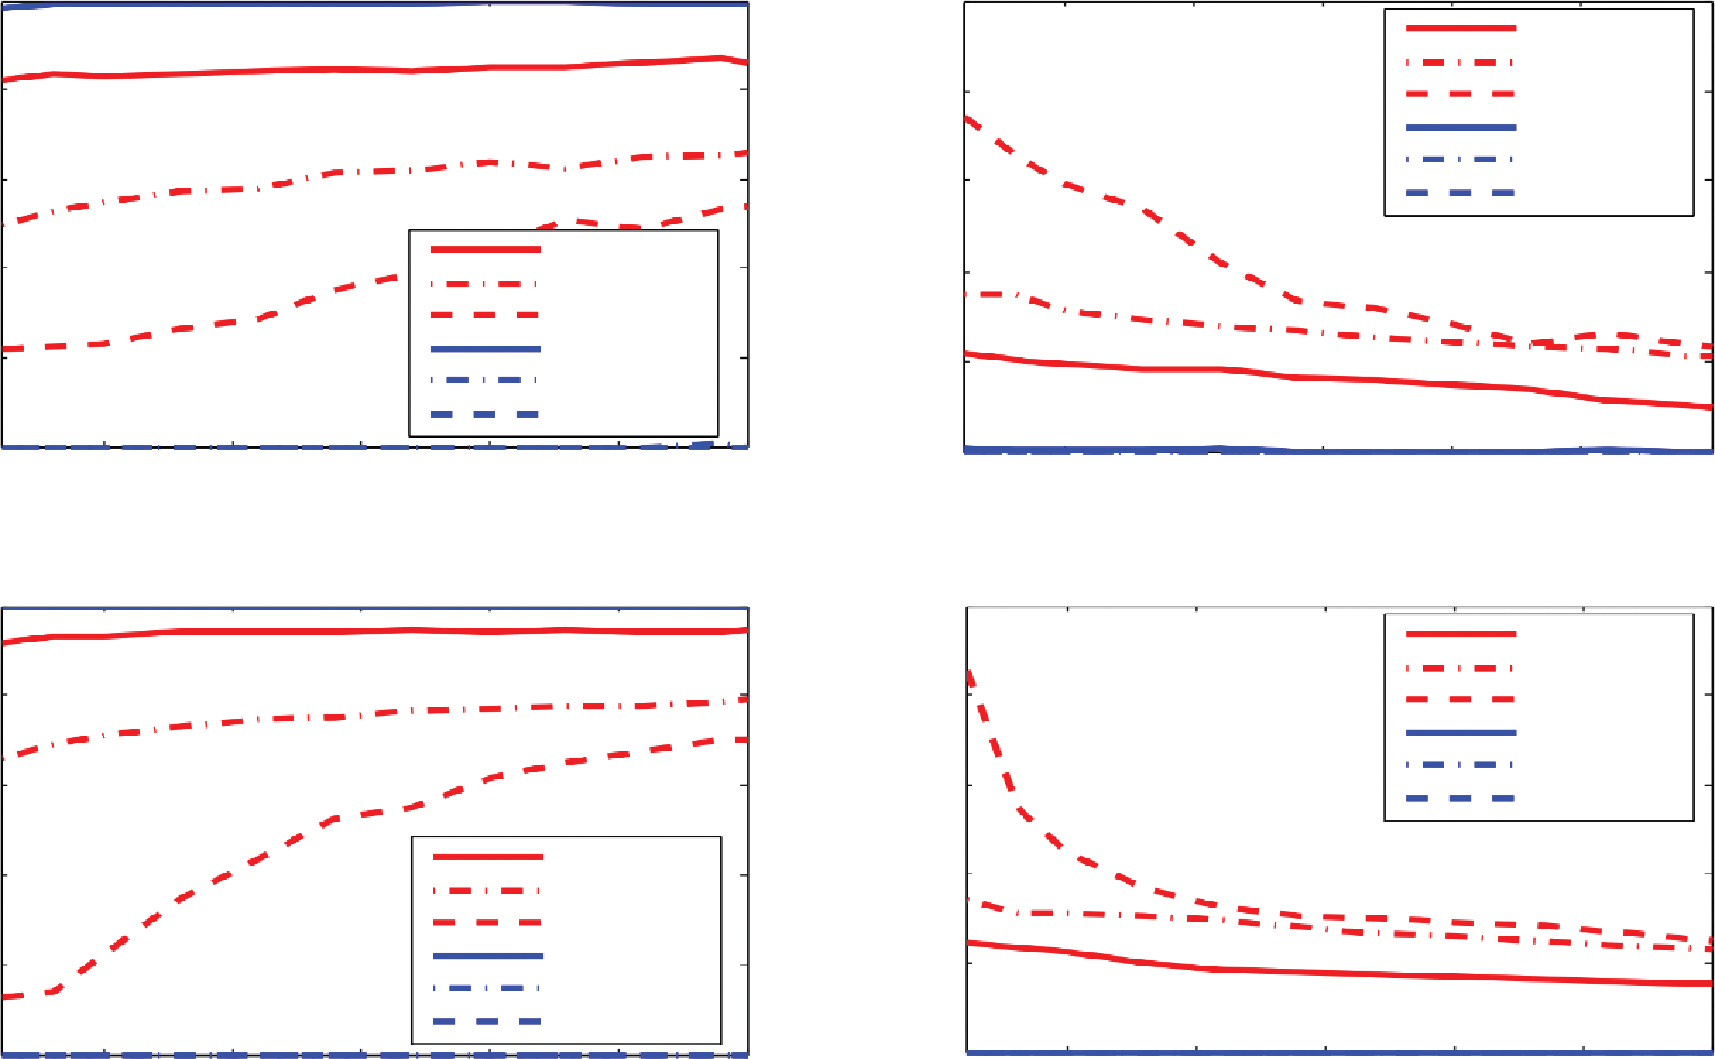
\includegraphics[width=137.2mm]{figures/ch01d_figure16_data.png}};
\node[font=\fontsize{7.0}{8}\selectfont] at (358.755,-29.070) {10 个表型，10 个 SNP：PD};
\node[font=\fontsize{7.0}{8}\selectfont] at (1324.962,-29.070) {10 个表型，10 个 SNP：FDR};
\node[font=\fontsize{7.0}{8}\selectfont] at (369.144,577.220) {30 个表型，30 个 SNP：PD};
\node[font=\fontsize{7.0}{8}\selectfont] at (1327.419,577.220) {30 个表型，30 个 SNP：FDR};
\node[rotate=90,font=\fontsize{7.0}{8}\selectfont] at (-75.867,224.994) {检出功效};
\node[rotate=90,font=\fontsize{7.0}{8}\selectfont] at (-75.867,832.723) {检出功效};
\node[font=\fontsize{7.0}{8}\selectfont] at (366.742,516.359) {样本量};
\node[font=\fontsize{7.0}{8}\selectfont] at (356.153,1119.854) {样本量};
\node[font=\fontsize{7.0}{8}\selectfont] at (1361.018,1119.854) {样本量};
\node[rotate=90,font=\fontsize{7.0}{8}\selectfont] at (889.461,840.340) {错误发现率};
\node[rotate=90,font=\fontsize{7.0}{8}\selectfont] at (889.461,234.179) {错误发现率};
\node[font=\fontsize{7.0}{8}\selectfont] at (-14.128,5.069) {1};
\node[font=\fontsize{7.0}{8}\selectfont] at (-26.496,94.094) {0.8};
\node[font=\fontsize{7.0}{8}\selectfont] at (-26.496,183.111) {0.6};
\node[font=\fontsize{7.0}{8}\selectfont] at (-26.496,272.135) {0.4};
\node[font=\fontsize{7.0}{8}\selectfont] at (-26.496,361.152) {0.2};
\node[font=\fontsize{7.0}{8}\selectfont] at (-14.128,450.177) {0};
\node[font=\fontsize{7.0}{8}\selectfont] at (945.553,5.069) {1};
\node[font=\fontsize{7.0}{8}\selectfont] at (933.185,94.093) {0.8};
\node[font=\fontsize{7.0}{8}\selectfont] at (933.185,183.111) {0.6};
\node[font=\fontsize{7.0}{8}\selectfont] at (933.185,272.135) {0.4};
\node[font=\fontsize{7.0}{8}\selectfont] at (933.185,361.152) {0.2};
\node[font=\fontsize{7.0}{8}\selectfont] at (945.553,454.412) {0};
\node[font=\fontsize{7.0}{8}\selectfont] at (949.789,610.685) {1};
\node[font=\fontsize{7.0}{8}\selectfont] at (937.420,699.706) {0.8};
\node[font=\fontsize{7.0}{8}\selectfont] at (937.420,788.727) {0.6};
\node[font=\fontsize{7.0}{8}\selectfont] at (937.420,877.747) {0.4};
\node[font=\fontsize{7.0}{8}\selectfont] at (937.420,966.768) {0.2};
\node[font=\fontsize{7.0}{8}\selectfont] at (949.789,1055.789) {0};
\node[font=\fontsize{7.0}{8}\selectfont] at (-15.534,610.685) {1};
\node[font=\fontsize{7.0}{8}\selectfont] at (-27.903,699.706) {0.8};
\node[font=\fontsize{7.0}{8}\selectfont] at (-27.903,788.726) {0.6};
\node[font=\fontsize{7.0}{8}\selectfont] at (-27.903,877.747) {0.4};
\node[font=\fontsize{7.0}{8}\selectfont] at (-27.903,966.768) {0.2};
\node[font=\fontsize{7.0}{8}\selectfont] at (-15.534,1055.789) {0};
\node[font=\fontsize{7.0}{8}\selectfont] at (1067.584,1081.927) {500};
\node[font=\fontsize{7.0}{8}\selectfont] at (1195.839,1081.927) {1000};
\node[font=\fontsize{7.0}{8}\selectfont] at (1324.092,1081.927) {1500};
\node[font=\fontsize{7.0}{8}\selectfont] at (1452.344,1081.927) {2000};
\node[font=\fontsize{7.0}{8}\selectfont] at (1580.603,1081.927) {2500};
\node[font=\fontsize{7.0}{8}\selectfont] at (1708.855,1081.927) {3000};
\node[font=\fontsize{7.0}{8}\selectfont] at (1361.017,516.362) {样本量};
\node[font=\fontsize{7.0}{8}\selectfont] at (1067.584,474.197) {500};
\node[font=\fontsize{7.0}{8}\selectfont] at (1195.839,474.197) {1000};
\node[font=\fontsize{7.0}{8}\selectfont] at (1324.092,474.197) {1500};
\node[font=\fontsize{7.0}{8}\selectfont] at (1452.344,474.197) {2000};
\node[font=\fontsize{7.0}{8}\selectfont] at (1580.603,474.197) {2500};
\node[font=\fontsize{7.0}{8}\selectfont] at (1708.855,474.197) {3000};
\node[font=\fontsize{7.0}{8}\selectfont] at (102.955,474.197) {500};
\node[font=\fontsize{7.0}{8}\selectfont] at (231.211,474.197) {1000};
\node[font=\fontsize{7.0}{8}\selectfont] at (359.466,474.197) {1500};
\node[font=\fontsize{7.0}{8}\selectfont] at (487.718,474.197) {2000};
\node[font=\fontsize{7.0}{8}\selectfont] at (615.970,474.197) {2500};
\node[font=\fontsize{7.0}{8}\selectfont] at (744.240,474.197) {3000};
\node[font=\fontsize{7.0}{8}\selectfont] at (102.955,1081.927) {500};
\node[font=\fontsize{7.0}{8}\selectfont] at (231.211,1081.927) {1000};
\node[font=\fontsize{7.0}{8}\selectfont] at (359.466,1081.927) {1500};
\node[font=\fontsize{7.0}{8}\selectfont] at (487.718,1081.927) {2000};
\node[font=\fontsize{7.0}{8}\selectfont] at (615.970,1081.927) {2500};
\node[font=\fontsize{7.0}{8}\selectfont] at (744.240,1081.927) {3000};
\node[anchor=west,font=\fontsize{5.6}{8}\selectfont] at (556.186,252.391) {S2SEM-常见};
\node[anchor=west,font=\fontsize{5.6}{8}\selectfont] at (556.186,285.648) {S2SEM-全部};
\node[anchor=west,font=\fontsize{5.6}{8}\selectfont] at (556.186,320.417) {S2SEM-罕见};
\node[anchor=west,font=\fontsize{5.6}{8}\selectfont] at (556.186,353.974) {SML-常见};
\node[anchor=west,font=\fontsize{5.6}{8}\selectfont] at (556.186,389.200) {SML-全部};
\node[anchor=west,font=\fontsize{5.6}{8}\selectfont] at (556.186,420.645) {SML-罕见};
\node[anchor=west,font=\fontsize{5.6}{8}\selectfont] at (556.186,856.592) {S2SEM-常见};
\node[anchor=west,font=\fontsize{5.6}{8}\selectfont] at (556.186,889.849) {S2SEM-全部};
\node[anchor=west,font=\fontsize{5.6}{8}\selectfont] at (556.186,924.618) {S2SEM-罕见};
\node[anchor=west,font=\fontsize{5.6}{8}\selectfont] at (556.186,958.173) {SML-常见};
\node[anchor=west,font=\fontsize{5.6}{8}\selectfont] at (556.186,993.399) {SML-全部};
\node[anchor=west,font=\fontsize{5.6}{8}\selectfont] at (556.186,1024.844) {SML-罕见};
\node[anchor=west,font=\fontsize{5.6}{8}\selectfont] at (1529.233,634.656) {S2SEM-常见};
\node[anchor=west,font=\fontsize{5.6}{8}\selectfont] at (1529.233,667.913) {S2SEM-全部};
\node[anchor=west,font=\fontsize{5.6}{8}\selectfont] at (1529.233,702.682) {S2SEM-罕见};
\node[anchor=west,font=\fontsize{5.6}{8}\selectfont] at (1529.233,736.242) {SML-常见};
\node[anchor=west,font=\fontsize{5.6}{8}\selectfont] at (1529.233,771.468) {SML-全部};
\node[anchor=west,font=\fontsize{5.6}{8}\selectfont] at (1529.233,802.913) {SML-罕见};
\node[anchor=west,font=\fontsize{5.6}{8}\selectfont] at (1532.054,29.042) {S2SEM-常见};
\node[anchor=west,font=\fontsize{5.6}{8}\selectfont] at (1532.054,62.299) {S2SEM-全部};
\node[anchor=west,font=\fontsize{5.6}{8}\selectfont] at (1532.054,97.068) {S2SEM-罕见};
\node[anchor=west,font=\fontsize{5.6}{8}\selectfont] at (1532.054,130.625) {SML-常见};
\node[anchor=west,font=\fontsize{5.6}{8}\selectfont] at (1532.054,165.849) {SML-全部};
\node[anchor=west,font=\fontsize{5.6}{8}\selectfont] at (1532.054,197.294) {SML-罕见};
\node[font=\fontsize{7.0}{8}\selectfont] at (-90.501,1165.288) {(c)};
\node[font=\fontsize{7.0}{8}\selectfont] at (-93.771,529.356) {(a)};
\node[font=\fontsize{7.0}{8}\selectfont] at (873.091,529.356) {(b)};
\node[font=\fontsize{7.0}{8}\selectfont] at (872.645,1163.174) {(d)};
\end{tikzpicture}
\origfig{16}{S2SEM 与 SML 推断表型网络的表现。分别在表型和基因型数目均为 10〔(a)、(b)〕及均为 30〔(c)、(d)〕时，比较两种方法的检出功效与错误发现率。图中“常见”“罕见”“全部”分别对应原图的 Com、Rare、All。}
\label{fig:omics-s2sem-sml}
\end{figure}
